\documentclass[A4,twoside]{ctexart}
%\usepackage{slashbox}\backslashbox
\usepackage{aappss}
%\renewcommand\baselinestretch{1.235}\protect
\renewcommand\baselinestretch{2.0}\protect
\abovedisplayshortskip 0 pt plus 3pt
\belowdisplayshortskip 6 pt plus 2pt minus 2pt
\abovedisplayskip 6 pt plus 2pt minus 2pt
\belowdisplayskip 6 pt plus 2pt minus 2pt
\newcommand{\mathd}{\mathrm{d}}
\newcommand{\supercite}[1]{\textsuperscript{\cite{#1}}}

% \info{2015}{64}{1}{01{}} \infodate{2015.0.0.}{2015.0.0.}
%=================== Text begin here ==============================

% ÕýÎÄ¿ªÊ¼

\begin{document}\apsname

\title{·ÇÍêÕûÁ¦Ñ§Óë¿ØÖÆ\fivestar}

\author{Íõ¶¨ÎÄ$^{1)\dag}$ \quad ¸ßÆÕÔÆ$^{1)}$}
\address{1)}{¹ú·À¿Æ¼¼´óѧ, º½Ìì¿ÆѧÓ빤³ÌѧԺ, ³¤É³ \quad 410072}

\abstract{·ÇÍêÕûÔ¼ÊøµÄ²»¿É»ýÐÔÊÇ·ÇÍêÕûÁ¦Ñ§µÄÀ§ÄÑËùÔÚ¡£¶ø·ÇÍêÕûÔ¼ÊøµÄÀ´Ô´ÊÇ·ÇÍêÕûÁ¦Ñ§Ñо¿Öг£±»ºöÊÓµÄÎÊÌâ¡£±¾ÎÄ´Ó·ÇÍêÕûÔ¼ÊøµÄÎïÀí±³¾°³ö·¢£¬½Òʾ³ö·ÇÍêÕûÁ¦Ñ§µÄ¿ØÖƱ¾ÖÊ¡£´Ó¿ØÖƵĹ۵ã¿ÉÒÔͳһ·ÇÍêÕûϵͳµÄ²»Í¬Ä£ÐÍ(ÈçChetaevÄ£ÐͺÍVaccoÄ£ÐÍ)¡£ÎÒÃÇÖ¸³ö·ÇÍêÕûÁ¦Ñ§ÈÔÈ»´¦ÓÚ·ÖÎöÁ¦Ñ§µÄÀíÂÛ¿ò¼ÜÄÚ£¬²»Í¬Ä£Ð͵ÄÇø±ð½öÔÚÓÚËüÃǸ÷×Ô°µº¬µÄ¿ØÖÆÁ¦²»Í¬¡£}

\keywords{·ÇÍêÕûÁ¦Ñ§£¬¿ØÖÆÂÛ£¬ChetaevÄ£ÐÍ£¬VaccoÄ£ÐÍ}

\pacs{45.05.+x,45.20.Jj,45.80.+r}

\cmail{wangdingwen0618@gmail.com \quad µç»°: 15116442661}


\section{ÒýÑÔ}
\label{sec:intr}
·ÇÍêÕûÁ¦Ñ§×÷Ϊ·ÖÎöÁ¦Ñ§µÄÒ»¸ö·ÖÖ¦£¬ÆäÑо¿¶ÔÏóÊÇÒ»ÀàÌØÊâµÄÁ¦Ñ§ÏµÍ³£¬¼´º¬·ÇÍêÕûÔ¼ÊøµÄϵͳ¡£Ò»°ãËù˵µÄ·ÇÍêÕûÔ¼ÊøÓÐÈçÏÂÐÎʽ£º
\begin{equation}
  \label{eq:nhcon}
  f_{\alpha}(\dot{q}_1,\dot{q}_2,\ldots,\dot{q}_n;q_1,q_2,\ldots,q_n;t)=0,\quad(\alpha=1,\ldots,m)
\end{equation}
ÆäÖÐ$q$ÊǹãÒå×ø±ê£¬$n$ÊǹãÒå×ø±êµÄÊýÄ¿£¬$m$ÊÇ·ÇÍêÕûÔ¼ÊøµÄÊýÄ¿¡£

ÔÚLagrange·¢Õ¹·ÖÎöÁ¦Ñ§Ê±²¢Ã»ÓзÇÍêÕûÔ¼ÊøµÄ¸ÅÄÔÚËûÄÇÀïËùνԼÊø¾ÍÊÇÖ¸¶Ôϵͳ×ø±êµÄÏÞÖÆ¡£Ö±µ½1894Ä꣬Hertz°ÑÈç\eqref{eq:nhcon}ÕâÑùµÄÔ¼ÊøÃüÃûΪ·ÇÍêÕûÔ¼Êø£¬´Ó´Ëµ®ÉúÁË·ÇÍêÕûÁ¦Ñ§\supercite{1}¡£¼òµ¥À´Ëµ£¬·ÇÍêÕûÔ¼ÊøµÄÌصãÊÇÔ¼Êø·½³ÌÖаüº¬×ø±êµÄµ¼Êý¶øÇÒµ¼ÊýÏî²»ÄÜͨ¹ý»ý·ÖµÄÊÖ¶ÎÏûÈ¥¡£

·ÖÎöÁ¦Ñ§ÖеÄÔ¼Êø»áµ¼ÖÂϵͳ×ÔÓɶÈÊý¼õÉÙ£¬Ê¹µÃºÜ¶à²»ÄÜ»òÄÑÓÚÓÃNewtonÁ¦Ñ§´¦ÀíµÄÎÊÌâµÃµ½½â¾ö£¬¶øÇÒÓÉ·ÖÎöÁ¦Ñ§·½·¨µÃµ½µÄ¶¯Á¦Ñ§·½³Ì¾ßÓÐÓë×ø±êÎ޹صÄÐÎʽ²»±äÐÔ£¬ÆäÒâÒåÒ²ÔçÒѳ¬³öÁ¦Ñ§·¶Î§¡£µ«ÔÚ·ÇÍêÕûÁ¦Ñ§ÖУ¬·ÇÍêÕûÔ¼ÊøµÄÒýÈëÈ´ÍùÍùʹÎÊÌâ¸ü¼Ó¸´ÔÓ¡£±ÈÈçÐéλÒÆÕâ¸öÔÚ·ÖÎöÁ¦Ñ§ÖÐÓÐ×Å»ù´¡µØλµÄ¸ÅÄÔÚ·ÇÍêÕûÁ¦Ñ§ÖÐÐèҪʩ¼Ó¶îÍâµÄÏÞÖÆÌõ¼þ²¢ÇÒСÐĵĶÔÆ䶨Òå²Å²»ÖÂÓÚÒý³öì¶Ü¡£Ò»°ãÈÏΪ·ÇÍêÕûÔ¼ÊøµÄÒýÈëËäȻʹµÃϵͳ×ÔÓɶÈÊý¼õÉÙ£¬µ«ÃèÊöϵͳÔ˶¯ËùÐèµÄ¹ãÒå×ø±êÊýÒª´óÓÚϵͳµÄ×ÔÓɶÈÊý¡£×ÔÓɶȵļõÉÙ²»½öûÓÐʹϵͳµÄÇó½â±äµÃÈÝÒ×£¬·´¶øʹµÃÎÊÌâ±äµÃÄÑÒÔÀí½â¡£¸ù¾Ý²»Í¬Á¦Ñ§Ä£Ð͸ø³öµÄÔ˶¯·½³ÌÍùÍù²»Ò»Ö£¬¸ü²»ÓÃ˵ËüÃǵÄÇó½âÁË\supercite{2,3,4}¡£

×ܵÄÀ´Ëµ£¬Ñо¿·ÇÍêÕûÁ¦Ñ§ÓÐÈýÌõ;¾¶£ºÒ»ÊÇ´Ó»ù±¾Ô­Àí³ö·¢£¬ÆÚÍûµÃµ½ÀàËÆÓÚ·ÖÎöÁ¦Ñ§ÖеÄLagrange·½³Ì»òHamiltonÕýÔò·½³ÌµÈÆÕ±éµÄÔ˶¯·½³Ì;ÁíÒ»·½Ïò¾ÍÊÇÀûÓÃÏÖ´ú΢·Ö¼¸ºÎµÄÓïÑÔÖØÐÂÃèÊö·ÇÍêÕûÁ¦Ñ§ÖеĸÅÄîºÍ¶¨Àí£¬ÒÔÆÚÀûÓü¸ºÎѧ·½·¨³¹µ×½â¾öÕâ¸öÎÊÌâ¡£µ«ÊÇ·ÇÍêÕûÔ¼ÊøϵͳÖеÄChetaevÄ£ÐͺÍVaccoÄ£ÐͲ¢²»µÈ¼Û£¬³¤ÆÚÒÔÀ´Ò»Ö±´æÔÚÕùÂÛ¡£¶øÏÖ´ú¼¸ºÎѧËäÈ»ÊÇÇ¿ÓÐÁ¦µÄ¹¤¾ß£¬È´²¢²»Äܽâ¾öеÄÎÊÌâ¡£Òò´Ë¸ü¼ÓÏÖʵµÄ;¾¶ÊÇÑо¿Ò»¸ö¸ö¾ßÌåµÄ·ÇÍêÕûϵͳµÄÀý×Ó¡£Õë¶Ôÿһ¸öʵÀýÁгöÆäÔ˶¯·½³Ì£¬²¢¶Ô·½³Ì½øÐÐÇó½â\supercite{5}¡£

ÒÔÒ»½×ÏßÐÔ·ÇÍêÕûÔ¼Êø
\begin{equation}
  \label{eq:linearnhcon}
    \sum_{j = 1}^n a_{\alpha j} ( q ; t) \dot{q}_j + b_i (q; t) = 0 \hspace{2em} ( \alpha =
  1, \cdots, m),
\end{equation}
ΪÀý£¬¶ÔÓÚÐéλÒÆ£¬Í¨³£ÈÏΪÓÐÈçϵĹØϵ³ÉÁ¢
\begin{equation}
  \label{eq:linearchetaev}
   \sum_{j = 1}^n a_{\alpha j} ( q ; t) \delta q_j = 0 \hspace{2em} ( \alpha = 1, \cdots, m).
\end{equation}
Ó¦ÓÃd'Alembert-LagrangeÔ­Àí,²¢ÒýÈëLagrange³Ë×Ó£¬µÃµ½ÈçϵÄÔ˶¯·½³Ì

\begin{equation}
  \label{eq:lineareom}
    \frac{\mathd}{\mathd t} \left( \frac{\partial L}{\partial \dot{q}_j}
   \right) - \frac{\partial L}{\partial q_j} = \sum_{\alpha = 1}^m \lambda_\alpha a_{\alpha
   j} \hspace{2em} ( j = 1, \cdots, n) .
\end{equation}
ÆäÖÐ$L$ÊÇϵͳµÄLagrangeº¯Êý¡£Õ⼸ºõÊDZê×¼µÄÇó½âÏßÐÔ·ÇÍêÕûÔ¼ÊøµÄ·½·¨£¬¿É¼ûÓںܶà·ÖÎöÁ¦Ñ§½Ì¿ÆÊé»ò·ÇÍêÕûÁ¦Ñ§×¨Öø\supercite{2,9,10}¡£

¶ÔÓÚÒ»°ãµÄ·ÇÏßÐÔ·ÇÍêÕûÔ¼Êø\eqref{eq:nhcon},ÒòΪÎÞ·¨µÃµ½ÐéλÒÆÖ®¼äµÄÏßÐÔ¹Øϵ£¬²»ÄÜÓ¦ÓóË×Ó·¨µÃµ½Ô˶¯·½³Ì¡£Ò»Ð©Ñо¿ÕßÈÏΪ£¬¿ÉÒÔÒýÈëÈçϵÄChetaevÌõ¼þ\supercite{2}£º
\begin{equation}
  \label{eq:chetaev}
 \sum_{j = 1}^n \frac{\partial f_\alpha}{\partial \dot{q}_j} \delta q_j=0\hspace{2em} ( \alpha = 1, \cdots, m),
\end{equation}
ÓÉ´Ë¿ÉÒԵõ½ÀàËÆÓÚ\eqref{eq:lineareom}µÄÔ˶¯·½³Ì
\begin{equation}
  \label{eq:leom}
    \frac{\mathd}{\mathd t} \left( \frac{\partial L}{\partial \dot{q}_j}
   \right) - \frac{\partial L}{\partial q_j} = \sum_{\alpha = 1}^m \lambda_\alpha \frac{\partial f_\alpha}{\partial \dot{q}_j} \hspace{2em} ( j = 1, \ldots, n) .
\end{equation}

µ«ÊÇÒ²ÓÐÑо¿Õß²»ÈÏͬChetaevÌõ¼þ,ËûÃÇ´ÓHamiltonÔ­Àí³ö·¢£¬Í¬ÑùÒýÈë²»¶¨³Ë×Ó£¬µÃµ½µÄÊÇÁíÍâÒ»×鶯Á¦Ñ§·½³Ì\supercite{6}
\begin{equation}
  \label{eq:eeom}
    \frac{\mathd}{\mathd t} \left( \frac{\partial L}{\partial \dot{q}_j}
   \right) - \frac{\partial L}{\partial q_j} = \sum_{\alpha = 1}^m\left[ \lambda_\alpha \left(\frac{\partial f_\alpha}{\partial q_j}-\frac{\mathd}{\mathd t} \frac{\partial f_\alpha}{\partial \dot{q}_j}\right)-\dot{\lambda}_\alpha \frac{\partial f_\alpha}{\partial \dot{q}_j}\right] \hspace{2em} ( j = 1, \ldots, n) £¬
\end{equation}
Õâ¾ÍÊÇͨ³£Ëù˵µÄVacco¶¯Á¦Ñ§Ä£ÐÍ¡£


ÓÉd'Alembert-LagrangeÔ­ÀíµÃµ½µÄ¶¯Á¦Ñ§·½³Ì\eqref{eq:leom}ºÍÓÉHamiltonÔ­ÀíµÃµ½µÄ¶¯Á¦Ñ§·½³Ì\eqref{eq:eeom}²¢²»ÏàÈÝ¡£¹ØÓÚÕâÁ½¸öÔ­ÀíË­¸üÊÊÓõÄÕùÂÛ£¬¹á´©ÓÚ·ÇÍêÕûÁ¦Ñ§·¢Õ¹µÄÕû¸ö¹ý³ÌÖС£Ò»°ãÈÏΪ£¬d'Alembert-LagrangeÔ­ÀíÒª±ÈHamiltonÔ­Àí¸üΪ»ù´¡\supercite{3,4}£¬ÆäÂÛÖ¤·½·¨Ö÷ÒªÊÇ£º1).ÒýÈëJourdanÔ­ÀíºÍGaussÔ­Àí£¬ÈÏΪͨ¹ýÕâÁ½ÖÖÔ­ÀíµÃµ½µÄÔ˶¯·½³ÌÓëd'Alembert-LagrangeÔ­ÀíµÃµ½µÄ·½³ÌÒ»Ö¡£2).ÊÔͼ´ÓÔ¼Êø·½³Ì³ö·¢À´Ö¤Ã÷ChetaevÌõ¼þ£¬¶ø²»ÊÇ°ÑËü×÷Ϊ¸½¼ÓµÄ¼ÙÉè¡£3).ÒÔNewtonÁ¦Ñ§×÷ΪÅжϱê×¼£¬½«Á½¸öÔ­ÀíµÃµ½µÄ¶¯Á¦Ñ§·½³ÌÓëÒÀ¾ÝNewtonÁ¦Ñ§µÃµ½µÄ·½³ÌÏà±È½Ï£¬´Ó¶ø¿Ï¶¨\eqref{eq:leom}¡£4).¹¹Ôì»òÑ°ÕÒ¸÷ÖÖʵÀý£¬ÂÛÖ¤d'Alembert-LagrangeÔ­ÀíµÃµ½µÄ¶¯Á¦Ñ§·½³ÌÓëÕæʵÀý×ÓµÄÔ˶¯Çé¿öÏà·û¡£


ÕâЩ¿Ï¶¨\eqref{eq:leom}¶ø·ñ¶¨\eqref{eq:eeom}µÄÀíÓɶ¼ÊǼä½ÓµÄ¡£Êµ¼ÊÉϲ»ÉÙѧÕ߶Ô\eqref{eq:leom}µÄ³ÉÁ¢´æÓÐÖÊÒÉ£¬ÒòΪÔÚ·ÇÏßÐÔ·ÇÍêÕûÔ¼ÊøÖÐÒýÈëµÄChetaevÌõ¼þ\eqref{eq:chetaev}ÊǺÁÎÞµÀÀíµÄ£¬Ëü²»ÄÜÓÉÔ¼Êø·½³ÌÍƳö¡£Æäʵ¼´Ê¹ÊÇÏßÐÔ·ÇÍêÕûϵͳ£¬Í¨³£ÈÏΪ×ÔÈ»³ÉÁ¢µÄ\eqref{eq:linearchetaev}Ò²ÓÐÎÊÌâ,ÓÉ\eqref{eq:linearnhcon}µ½\eqref{eq:linearchetaev}µÄÀíÓÉÊÇËÆÊǶø·ÇµÄ¡£Êµ¼ÊÉÏ£¬Èç¹û¶ÔÏßÐÔÔ¼Êø·½³Ì\eqref{eq:linearnhcon}½øÐбä·ÖÔËË㣬µÃµ½µÄÓ¦ÊÇÈçÏ·½³Ì
\begin{equation}
 \sum_{j = 1}^n a_{\alpha j}  \delta \dot{ q}_j +  \sum_{j = 1,k=1}^n \frac{\partial a_{\alpha j} }{\partial q_k} \dot{ q}_j \delta q_k +\sum_{k=1}^n \frac{\partial b_\alpha }{\partial q_k}\delta q_k = 0 \hspace{2em} ( \alpha = 1, \cdots, k).
\end{equation}

ÁíÍ⣬ӦÓÃChetaevÄ£ÐͲ»¿É±ÜÃâµÄÅöµ½·ÇÍêÕûÔ¼ÊøÁ¦µÄÎïÀíÒâÒåÎÊÌâ¡£Ô¼Êø·½³Ì¶ÔÓ¦×ÅÔ¼ÊøÁ¦£¬¶øÕâ¸öÔ¼ÊøÁ¦¾¿¾¹ÈçºÎʵÏÖÒÔ¼°ËüµÄÎïÀíʵÖÊÊÇʲôÔÚChetaevÄ£ÐÍÖв¢Ã»Óеõ½ºÜºÃµÄ»Ø´ð¡£ÔÚ·ÇÍêÕûÁ¦Ñ§ÖÐһϵÁйØÓÚÐéλÒƵĶ¨Ò塢΢·Ö-±ä·ÖµÄ½»»»¹ØϵºÍ±ä·ÖÔ­ÀíÊÊÓÃÐԵȲ»Í¬ÈÏʶÕýÔ´ÓÚ¶ÔÔ¼Êø·½³Ì¼°ÆäÔ¼ÊøÁ¦ÈÏʶµÄ²»×ã\supercite{8}¡£

·ÇÍêÕûÁ¦Ñ§±ØÐè»Ø´ðÈçÏÂÎÊÌ⣺×÷Ϊ·ÖÎöÁ¦Ñ§»ù´¡µÄÁ¦Ñ§Ô­ÀíºÍ»ù±¾¸ÅÄî¶ÔÓÚ·ÇÍêÕûϵͳÊÇ·ñÈÔÈ»³ÉÁ¢£¿ÎÒÃÇÈÏΪÕâ¸öÎÊÌâµÄ´ð°¸£¬ÐèÒª´Ó·ÇÍêÕûϵͳµÄÎïÀí±¾ÖÊÖÐÑ°ÕÒ¡£±¾ÎIJ¢²»´òËãÕë¶Ô·ÇÍêÕûϵͳ¸ø³öеıä·ÖÔ­Àí»òÔ˶¯·½³Ì£¬¶øÊÇÊÔͼ²ûÃ÷ÈçϹ۵㣺·ÇÍêÕûÁ¦Ñ§²¢²»³¬³ö·ÖÎöÁ¦Ñ§ÖÐÁ¦Ñ§Ô­ÀíµÄÊÊÓ÷¶Î§;·ÇÍêÕûÁ¦Ñ§ÖдæÔÚµÄһЩì¶ÜºÍÕùÂÛ£¬ÊÇÓÉÓÚ¶ÔϵͳģÐ͵Ĺý¶È¼ò»¯ºÍ¶ÔϵͳµÄ²»ÍêÈ«ÃèÊöµ¼ÖµÄ;Ëùν·ÇÍêÕûÔ¼Êø²»¾ß±¸ÍêÕûÔ¼ÊøÔÚ·ÖÎöÁ¦Ñ§ÖеĻù´¡µØ룬·ÇÍêÕûÁ¦Ñ§ÎÊÌâ±¾ÖÊÉÏÊÇÓë¿ØÖÆÎÊÌâÃܲ»¿É·ÖµÄ£¬ÍÑÀëÁË¿ØÖƱ³¾°µÄ·ÇÍêÕûÔ¼ÊøÊDz»´æÔڵġ£

½«¿ØÖÆÂÛÓë·ÇÍêÕûÁ¦Ñ§ÁªÏµÔÚÒ»ÆðµÄ¹Ûµã²¢²»ÐÂÏÊ\supercite{7}£¬Ò²ÔçÓÐѧÕßÈÏʶµ½½ö¸ø³öÔ¼Êø·½³Ì¶øÎïÀí±³¾°Î´¸ø³öµÄÁ¦Ñ§ÏµÍ³ÊÇ¡°²»Í걸Á¦Ñ§ÏµÍ³¡±»ò¡°²»È·¶¨Á¦Ñ§ÏµÍ³¡±\supercite{8}¡£µ«ÎÒÃÇÈÏΪ¾­µä·ÇÍêÕûϵͳÃèÊöµÄ²»ÍêÈ«ÐÔÒÔ¼°ËüµÄ¿ØÖƱ¾ÖÊÊÇ·ÇÍêÕûÁ¦Ñ§µÄºËÐÄÎÊÌâ¡£·ÇÍêÕûÁ¦Ñ§ÖеÄһЩÒýÆðÕùÒéºÍ²»Í¬ÈÏʶµÄ¹ÛµãÈçÐéλÒƵĶ¨ÒåÎÊÌ⣬΢·ÖÓë±ä·ÖµÄ½»»»¹ØϵÎÊÌâÒÔ¼°Ô¼Êø·½³ÌºÍÔ¼ÊøÁ¦¹ØϵÎÊÌⶼÓë´ËÃܲ»¿É·Ö¡£ÈÏʶµ½ÕâÒ»µã£¬ÎÒÃǾͻᷢÏÖ·ÇÍêÕûÁ¦Ñ§²»Í¬Ä£ÐÍÖ®¼ä²»µÈ¼ÛµÄÔ­ÒòËùÔÚ¡£¸ü½øÒ»²½£¬ÎÒÃÇÒ²½«Òâʶµ½·ÇÍêÕûÁ¦Ñ§ÈÔ´¦ÓÚ·ÖÎöÁ¦Ñ§µÄÀíÂÛ¿ò¼ÜÖ®ÖС£

\section{Ô¼ÊøÊÇʲô£¿}
\label{sec:constraint}


·ÖÎöÁ¦Ñ§Ñо¿µÄÖ÷ÒªÊǺ¬Ô¼ÊøµÄÁ¦Ñ§ÏµÍ³¡£µ«ÔÚLagrange·¢Õ¹·ÖÎöÁ¦Ñ§Ê±£¬Ö»¿¼ÂÇÁ˶ÔϵͳλÐεÄÔ¼Êø£¬Ò²¾ÍÊǺóÀ´Ëù˵µÄÍêÕûÔ¼Êø¡£Ö±µ½Ò»¸ö¶àÊÀ¼Íºó£¬Hertz²ÅÕýʽÌá³öÁË·ÇÍêÕûÔ¼ÊøµÄ¸ÅÄ´Ó¶ø¿ª´´ÁË·ÇÍêÕûϵͳ¶¯Á¦Ñ§ÕâÒ»ÁìÓò¡£

×Ô´Ó·ÇÍêÕûÔ¼ÊøµÄ¸ÅÄîÌá³öÒÔÀ´£¬¹ØÓÚËüµÄÕùÂÛ¾ÍûÓÐÍ£Ö¹¹ý¡£ËäÈ»·ÇÍêÕûÔ¼ÊøÊÇÒ»´óÀàÔ¼Êø£¬µ«ÊÇÔÚʵ¼ÊÓ¦ÓÃÖУ¬·ÇÍêÕûϵͳµÄ¶¯Á¦Ñ§·½³ÌºÜÉÙ±»Ê¹Ó᣹۲ìһЩµäÐ͵ķÇÍêÕûϵͳ¿ÉÒÔ·¢ÏÖ£¬·ÇÍêÕûÔ¼ÊøÒ»°ã´æÔÚÓÚÓøÕÌåÄ£ÐÍÃèÊöµÄϵͳÖÐ;¶ø¶ÔÓÚ΢¹Ûϵͳ£¬²¢Ã»ÓÐÓõ½·ÇÍêÕûÔ¼ÊøµÄ¸ÅÄî¡£ÀýÈç¸ÕÌå´¿¹ö¶¯ÊǵäÐ͵ķÇÍêÕûÔ¼Êø£¬Ò»¸öÖªÃûÀý×Ó¾ÍÊÇ·ÒÀ¼Ñ§ÕßLindel\"of¶Ô»ØתÃæ¸ÕÌåÑØˮƽÃæ´¿¹ö¶¯µÄÑо¿¡£µ«´¿¹ö¶¯Ö»ÊÇÒ»ÖÖ¼ÙÉ裬ÓÉ´¿¹ö¶¯Òý³öµÄ·ÇÍêÕûÔ¼Êø¸ÅÄîÓÐ×ÅŨºñµÄÈËΪºÛ¼£¡£ÊÂʵÉÏ£¬Ò»Ð©·ÇÍêÕûÁ¦Ñ§¾­µäÀý×ÓÍùÍù¸øÈËÒ»ÖÖÊÇΪÁ˵õ½·ÇÍêÕûÔ¼Êø´Ó¶ø¹ÊÒâ¹¹Ôì³öÀ´µÄÓ¡Ïó\supercite{2}¡£

ÍêÕûÔ¼ÊøÓÐÏÊÃ÷µÄÎïÀíͼÏó£¬ÔÚDescartes×ø±êϵÏ£¬Ëü¾ÍÊǶÔÖʵã»òÖʵãϵλÖõÄÔ¼Êø¡£µ±Ô¼ÊøÊÇÀíÏëÔ¼Êøʱ£¬Ó¦ÓÃd'Alembert-LagrangeÔ­Àí£¬¿ÉÒԵõ½ÏµÍ³µÄLagrange·½³Ì¡£ÓÉÓÚÒýÈëÁËLagrangeº¯Êý£¬Ê¹µÃ·½³Ì¶Ô²»Í¬µÄÒ»×é¹ãÒå×ø±ê¾ßÓÐÐÎʽ²»±äÐÔ¡£LagrangeÁ¦Ñ§µÄ¹Ø¼üÖ®´¦ÊǹãÒå×ø±êµÄÒýÈë¡£ÀûÓÃÇ¡µ±µÄ¹ãÒå×ø±ê£¬¿ÉÒÔʹԼÊøÌõ¼þ×ÔÈ»µÃµ½Âú×㣬ÄÇôÔÚ½ÓÏÂÀ´µÄ·ÖÎöÖпÉÒÔ²»¿¼ÂÇÔ¼ÊøµÄ×÷Ó㬴Ӷø¼ò»¯ÁËÎÊÌâ¡£Èç¹ûÒªµÃµ½Ô¼ÊøÁ¦£¬Ò²Ö»ÐèÀûÓÃLagrange³Ë×Ó·¨£¬½â³öµÄ³Ë×ÓÕýºÃ¶ÔÓ¦×ÅÔ¼ÊøÁ¦¡£

LagrangeµÄ·ÖÎöÁ¦Ñ§ÌåÏÖ³öÒ»ÖÖ¼ò½àºÍÃÀ¸Ð¡£µ«µ±·ÇÍêÕûÔ¼Êø´æÔÚµÄʱºò£¬ÎÊÌâµÄ´¦Àí±äµÃ¸´ÔÓÆðÀ´¡£½ü°ÙÄêÀ´£¬ÈËÃǶԷÇÍêÕûϵͳ×öÁË´óÁ¿Ñо¿£¬µÃµ½Á˸÷ʽ¸÷ÑùµÄÔ˶¯·½³Ì¡£µ«ÈËÃǶԴËÎÊÌâÈÔ²»ÄÜÓÐÒ»ÖµÄÈÏʶ£¬¶Ô·ÇÍêÕûϵͳÊÊÓõÄÁ¦Ñ§Ô­ÀíÒÔ¼°µÃµ½µÄÔ˶¯·½³ÌµÄÓÐЧÐÔ»¹´æÔÚÕùÂÛ¡£´ËÍ⣬ÎÞÂÛʹÓÃd'Alembert-LagrangeÔ­Àí»¹ÊÇHamiltonÔ­Àí£¬ËùµÃµ½µÄÔ˶¯·½³Ì¶¼Ê®·Ö·±¸´£¬ºÜÄÑÏëÏóËüÃÇÄܹ»ÓÐ×Åʵ¼ÊµÄÓ¦Óá£

ÕâЩÎÊÌâµÄ´æÔÚ£¬´ÙʹÎÒÃǶԷÇÍêÕûÔ¼ÊøÐèÒªÖØÐÂÉóÊÓ£¬ÆäÖÐÊ×ÒªµÄ¾ÍÊǶÔÔ¼ÊøµÄÎïÀíÒâÒå½øÐзÖÎö¡£
LagrangeËù·¢Õ¹µÄ·ÖÎöÁ¦Ñ§²»Í¬ÓÚNewtonÁ¦Ñ§¡£NewtonÁ¦Ñ§Êµ¼ÊÉÏ´¦ÀíµÄÊÇÖʵãµÄÔ˶¯£¬¶ø·ÖÎöÁ¦Ñ§Ëù¿¼ÂǵĶÔÏó»ù±¾ÉÏÊÇÒ»¸öº¬Ô¼ÊøµÄϵͳ£¬Ò²¾ÍÊÇ˵ÊÇÖʵã¼äÓÐÒ»¶¨Î»ÖùØϵµÄÖʵãϵ¡£ÈçҪʹÓÃNewtonÁ¦Ñ§Çó½âÖʵãϵµÄÔ˶¯ÐèÒªÖªµÀÿ¸öÖʵãËùÊܵ½µÄÁ¦£¬²¢ÇÒÖªµÀϵͳµÄ³õ״̬¡£µ«Ëæ×ÅϵͳÖеÄÖʵãÊýÔö¶à£¬¶øÇÒÖʵã¼ä»¹´æÔÚ´óÁ¿µÄÏ໥×÷Óã¬ÕâЩÏ໥×÷ÓöÔÿ¸öÖʵã²úÉúµÄÁ¦ÍùÍù²»Äܹ»Ô¤ÏÈÖªµÀ£¬ÓÉ´ËʹµÃÖʵãϵµÄÔ˶¯ÔÚNewtonÁ¦Ñ§¿ò¼ÜÏÂʵ¼ÊÉϲ»¿É½â¡£

ΪÁËÄܶÔʵ¼ÊµÄÎÊÌâ½øÐÐÀíÂÛ·ÖÎö£¬ÈËÃǸù¾ÝËù´¦ÀíµÄ¶ÔÏóµÄÌص㣬ÍùÍù¶Ôϵͳ×öÁË´óÁ¿µÄ¼ò»¯ºÍ¼ÙÉè¡£¶øÕâЩ¼ò»¯Óë¼ÙÉèʵ¼Ê¾ÍÊÇÔ¼ÊøµÄÒýÈë¡£ÔÚ¾­µäÁ¦Ñ§µÄ·¶³ëÄÚ£¬¿ÉÒÔ¸ù¾ÝÔ¼ÊøÇé¿ö½«Á¦Ñ§ÏµÍ³·ÖΪÈçÏÂÈýÀà¡£

1.ÖʵãÊý½ÏÉÙ»òÖʵã¼äÓÐ׏̶¨Î»ÖùØϵµÄϵͳ¡£¸ÕÌåÁ¦Ñ§¡¢ÌìÌåÁ¦Ñ§Ëù´¦ÀíµÄÕýÊÇÕâÀà¶ÔÏó¡£ÕâÀàϵͳµÄÌصãÊÇϵͳ±äÁ¿²»Ì«¶à£¬¼´ÏµÍ³×ÔÓɶȽÏÉÙ£¬ÏµÍ³¿ÉÒÔÓÃÖʵãÄ£Ðͺ͸ÕÌåÄ£ÐÍ»òÕâЩģÐ͵Ä×éºÏÓëµþ¼ÓÀ´ÃèÊö¡£

2.Öʵã¼äλÖùØϵ»ù±¾¹Ì¶¨£¬µ«Öʵã¼äÒ²¿ÉÒÔÓÐÏà¶ÔÔ˶¯¡£Õñ¶¯ÎÊÌâÒÔ¼°¹ÌÌåÁ¦Ñ§Ñо¿µÄ¶ÔÏ󶼿ÉÒÔ¹éÓÚÕâÀàϵͳ¡£ÕâÀàϵͳ×ÔÓɶÈÊÇÎÞÏ޵ģ¬µ«Ã¿¸öÖʵã¿ÉÒÔÈÏΪֻÊÇÔÚ»ù׼λÖø½½üÔ˶¯¡£»òÕßÊÇ×öÍù¸´Ô˶¯£¬Õâ¾ÍÊÇÕñ¶¯ÎÊÌâ;»òÕßÊÇÖʵãλÖÃÆ«ÀëÒ»¶¨³Ì¶È£¬Õâ¾ÍÊǵ¯ÐÔÐαäÎÊÌâ¡£

3.Öʵã¼äλÖò»¹Ì¶¨£¬´æÔÚ×Å´óÁ¿ÅöײºÍÏ໥×÷Óá£ÈÈÁ¦Ñ§£¬Í³¼ÆÁ¦Ñ§Ñо¿µÄÕýÊÇÕâÀàϵͳ¡£ÕâÀàϵͳµÄ×ÔÓɶÈÒ²¿ÉÒÔ¿´×÷ÊÇÎÞÏ޵ģ¬ÈËÃÇÎÞ·¨ÖªµÀϵͳÄÚ¾ßÌåij¸öÖʵãµÄÔ˶¯×´Ì¬£¬¶øÖ»ÊÇÑо¿ÏµÍ³ºê¹ÛºÍƽ¾ùµÄÐÔÖÊ£¬Æ©Èçζȡ£Á÷ÌåÁ¦Ñ§Ñо¿µÄ¶ÔÏó½éÓÚµÚ¶þÀàºÍµÚÈýÀàϵͳ֮¼ä¡£

°Ñϵͳ°´×ÔÓɶÈÊýµÄÇé¿ö·ÖÀ࣬ʵ¼ÊÉÏÒ²ÊÇ°´ÏµÍ³ÄÚ²¿Ô¼ÊøÇé¿ö·ÖÀà¡£ÕâÀïµÄÔ¼ÊøÖ¸¶ÔÖʵãλÖùØϵµÄÔ¼Êø£¬Ò²¾ÍÊÇͨ³£Ëù˵µÄÍêÕûÔ¼Êø¡£ÍêÕûÔ¼ÊøµÄ¸ÅÄîÊǺÜ×ÔÈ»µÄ£¬ÔÚHertz·Ö±æ³ö·ÇÍêÕûÔ¼Êø֮ǰÈËÃÇËù˵µÄÔ¼Êø½öÖ¸ÍêÕûÔ¼Êø¡£·ÇÍêÕûÔ¼ÊøµÄ¸ÅÄîÆðÔ´ÓÚº¬¸ÕÌåµÄϵͳ£¬Ò²¾ÍÊÇÉÏÊöµÚÒ»Ààϵͳ£¬ÕâÀàϵͳµÄÌصãÊÇ×ÔÓɶÈÓÐÏÞ¡£ÕâÒ²¾ö¶¨ÁË·ÇÍêÕûÔ¼ÊøµÄ¸ÅÄî¼°Æä¾ßÌåÐÎʽ¸ü¶àµÄÊÇÒ»ÖÖ¼ÙÉèºÍ¶ÔÕæʵÔ˶¯µÄÒ»Öֱƽü£¬²¢Ã»ÓоßÌåµÄÎïÀí¹æÂɱ£Ö¤·ÇÍêÕûÔ¼ÊøµÄ³ÉÁ¢¡£±¾ÎĽ«Òª±íÃ÷£¬ËùνµÄ·ÇÍêÕûÁ¦Ñ§ÎÊÌâ±¾ÖÊÉÏÓë¿ØÖÆÎÊÌâ²»¿É·ÖÀ룬·ÇÍêÕûÔ¼ÊøÊÇÓÉÓÚÍâ½çÊ©¼ÓµÄ¿ØÖƵ¼Öµģ¬¼´·ÇÍêÕûÔ¼ÊøÓ¦µ±ÊÓΪ¿ØÖƵĽá¹û¡£´ÓÕâ¸öÒâÒåÉÏ˵£¬·ÇÍêÕûÔ¼ÊøÊÇÒ»ÖÖ¡°²»×ÔÈ»¡±µÄÔ¼Êø£¬Æä±¾Éí¾Í·´Ó³ÁËÔ˶¯¹æÂÉ£¬´Ó¶øÓëÍêÕûÔ¼ÊøÓб¾ÖʵIJ»Í¬¡£

¾­µäµÄ·ÇÍêÕûÔ¼ÊøÀý×Ó¶¼Óë¸ÕÌåÔ˶¯Óйأ¬ÀýÈç±ùµ¶Ô˶¯ÎÊÌâ¡¢Á½ÂÖС³µÎÊÌâ¡¢¸ÕÇòÔÚ´Ö²ÚƽÃæ¹ö¶¯ÎÊÌâµÈ¡£ÕâЩϵͳÃèÊöÆðÀ´·Ç³£¼òµ¥£¬µ«ÊÇÆäÇó½â³£³£Ê®·ÖÀ§ÄÑ£¬ËùµÃµÄ½âÒ²ÍùÍù¾­²»ÆðÍÆÇá£ÔÚÏÂÒ»½ÚÎÒÃǽ«Ïêϸ·ÖÎö±ùµ¶Ô˶¯Õâ¸ö¾­µäµÄ·ÇÍêÕûϵͳ£¬²¢ÒÔ´ËΪÀý³ÎÇåһЩÔÚ·ÇÍêÕûÁ¦Ñ§Ñо¿Öо­³£»áÓöµ½µÄÎóÇø£¬²¢¶Ô·ÇÍêÕûÔ¼ÊøµÄÀ´Ô´½øÐÐ̽ÌÖ¡£

\section{±ùµ¶Ô˶¯}
\label{sec:ice}
\newtheorem{example}{Àý}

\begin{example}
  ±ùµ¶Ôڹ⻬ˮƽ±ùÃæÉÏÔ˶¯¡£¿ÉÒÔÓÃϸ¸ËΪģÐÍÃèÊö±ùµ¶ÃæµÄÔ˶¯£¬ÔÚÔ˶¯¹ý³ÌÖиËÉϵÄÒ»µã$C$£¨¿ÉȡΪÖÊÐÄ£©Ê¼ÖÕÑØן˵ķ½Ïò¡£ÔÚƽÃæÉϽ¨Á¢×ø±êϵ£¬$Oz$ÖáÊúÖ±ÏòÉÏ£¬¸ËÔÚ$xOy$ƽÃæÄÚÔ˶¯¡£ÓÃÀ´ÃèÊöÕâ¸ö¸ËÔ˶¯µÄÈý¸ö¹ãÒå×ø±ê¿ÉѡΪ$x,y,\varphi$,ÆäÖÐ$\varphi$ÊǸËÓë$Ox$ÖáµÄ¼Ð½Ç¡£
\end{example}

´Ëϵͳ¿ÉÒÔÈÏΪÊܵ½Á½¸öÔ¼Êø£¬·Ö±ðÊÇÍêÕûÔ¼Êø
\begin{equation}
  \label{eq:ice1}
  z = 0
\end{equation}
ºÍ·ÇÍêÕûÔ¼Êø
\begin{equation}
  \label{eq:ice2}
  \dot{x} \sin\varphi - \dot{y} \cos\varphi = 0
\end{equation}

Éè$m$ÊDZùµ¶µÄÖÊÁ¿£¬$I_C$ÊDZùµ¶¶Ô¹ýÖÊÐĵÄÊúÖ±ÖáµÄ¹ßÐԾأ¬Ôò±ùµ¶µÄ¶¯ÄܿɱíʾΪ
\begin{equation}
  \label{eq:ice3}
  T = \frac{1}{2}m\left(\dot{x}^2+\dot{y}^2\right)+\frac{1}{2}I_C\dot{\varphi}^2.
\end{equation}
±ùÃæ¹â»¬ÎÞĦ²Á£¬²¢ÇÒ±ùµ¶ÖØÁ¦ÊÆÄÜΪ³£Êý£¬ÀûÓÃChetaevλÒƼÙÉ裬¾ÍµÃµ½ÈçϵÄÔ˶¯·½³Ì
\begin{equation}
  \label{eq:iceeom}
  m \ddot{x} = \lambda \sin\varphi, m \ddot{y} = -\lambda \cos\varphi, \ddot{\varphi} = 0.
\end{equation}
ÆäÖÐ$\lambda$ÊÇÒýÈëµÄLagrange³Ë×Ó¡£
¼ÙÉè³õʼʱ¿Ì±ùµ¶ÖÊÐÄλÓÚÔ­µã£¬±ùµ¶ÑØ×Å$Ox$ÖᣬÖÊÐijõËÙ¶ÈΪ$v_0$,±ùµ¶½ÇËÙ¶ÈΪ$\omega_0$.´Ëʱ¿ÉµÃ·½³ÌµÄ½âΪ
\begin{equation}
  \label{eq:icesol}
  x(t) = \frac{v_0}{\omega_0}\sin\omega_0t, y(t) = \frac{v_0}{\omega_0}(1 - \cos\omega_0t), \varphi(t) = \omega_0
\end{equation}
Òò´Ë£¬±ùµ¶ÖÊÐÄÒÔËÙ¶È$v_0$ÈÆÖÐÐÄλÓÚ$Oy$ÖáÉϰ뾶Ϊ$v_0/\omega_0$µÄÔ²ÖܵÈËÙת¶¯¡£

´ËʱLagrange³Ë×ÓÒ²¿ÉÒÔ´Ó\eqref{eq:iceeom}ÖÐÇó³ö£º
\begin{equation}
  \label{eq:icel}
 \lambda = -m\omega_0v_0
\end{equation}
´Ë$\lambda$ÕýÊÇÔ¼Êø·´Á¦$\mathbf{R}$.´ËÔ¼Êø·´Á¦ÔÚ$Ox$ÖáºÍ$Oy$ÖáµÄͶӰΪ$R_x$ºÍ$R_y$.
\begin{equation}
  \label{eq:icecon}
  R_x = -m_0\omega_0v_0\sin\omega_0t, R_y = m \omega_0v_0\cos\omega_0t
\end{equation}

Ô¼Êø·´Á¦´óСΪ³£Öµ£¬·½ÏòÖ¸Ïò±ùµ¶ÖÊÐÄÔ˶¯¹ì¼£µÄÔ²ÐÄ¡£
ÕâÊǽ̿ÆÊéÉϹØÓÚ´ËÎÊÌâµÄ±ê×¼½â·¨\supercite{9,10}¡£µ«ÊÇ×Ðϸ·ÖÎöÕâ¸ö½â´ð¹ý³Ì£¬È´·¢ÏÖÓÐÐí¶àÐèÒªÍÆÇõĵط½¡£

×îÒª½ôµÄÊÇÐèҪ˵Ã÷±ùµ¶×öÔ²ÖÜÔ˶¯ËùÐèÏòÐÄÁ¦µÄÎïÀíÒâÒå¡£Ò»¸ö×ÔÈ»µÄ½âÊÍÊÇÕâ¸öÏòÐÄÁ¦¾ÍÊDZùÃæ¶Ô±ùµ¶µÄÔ¼Êø·´Á¦£¬Õâ¸öÔ¼Êø·´Á¦¶ÔÓ¦×Å·ÇÍêÕûÔ¼Êø\eqref{eq:ice2}¡£µ«ÎÒÃÇÒѼÙÉè±ùÃæÊǹ⻬µÄ£¬Ò²¼´²»¿¼ÂÇĦ²ÁÒòËØ£¬±ùÃæ³ýÁ˸ø±ùµ¶ÒÔÖ§³ÅÁ¦£¬µ½µ×ͨ¹ýºÎÖÖ×÷ÓÃÌṩԲÖÜÔ˶¯ËùÐèµÄÏòÐÄÁ¦£¿
ºÜ¶à×÷Õ߶ÔÕâ¸öÁ¦µÄÐÔÖʽøÐÐÁË̽ÌÖ,һЩѧÕßÖ±½Ó³ÆÆäΪ¡°·ÇÍêÕûÁ¦¡±¡£¹ùÖÙºâ\supercite{6}ÔòÈÏΪ±ùµ¶×öÔ²ÖÜÔ˶¯ÐèÒªÓÐÒ»¸öÍâ¼ÓµÄ¸úËæÁ¦£¬Èô²»Ê©¼Ó´ËÁ¦±ùµ¶Ö»ÄÜ×÷Ö±ÏßÔ˶¯¡£±ØÐè×¢ÒâµÄÊÇÕâ¸ö¸úËæÁ¦±ØÐèÃ÷È·¸ø¶¨£¬¶ø²»ÊǺ¬»ì²»ÇåµÄ¡°·ÇÍêÕûÁ¦¡±¡£

ÁíÒ»¸öÖµµÃ¹Ø×¢µÄÎÊÌâÊDZùµ¶µÄ·ÇÍêÕûÔ¼Êø¾¿¾¹ÈçºÎʵÏÖ£¿\eqref{eq:ice2}ÊǶԱùµ¶ÃæÉϵÄÿһµã³ÉÁ¢£¬»¹Êǽö½ö¶ÔÖÊÐÄ»ò½Ó´¥µã³ÉÁ¢£¿Èç¹ûÊÇÇ°Õߣ¬ÔòÒ»·½Ãæ±ùµ¶ÉϵÄËùÓеãÒªÑØ×űùµ¶Ãæ¸ø³öµÄ·½ÏòÔ˶¯£¬Õâ¾ÍÒªÇó±ùµ¶²»µÃÓÐÈÆ×ÔÉíÊúÖ±ÖáµÄת¶¯£¬¶øÁíÒ»·½ÃæÒѽâµÃ±ùµ¶ÖÊÐÄ×÷Ô²ÖÜÔ˶¯£¬±ùµ¶ÓÖÈÆÆäÖÊÐÄ×ÔÓÉÐýת£¨$\varphi(t)=\omega_0$£©¡£ÏÔÈ»£¬ÕâÁ½·½ÃæÎÞ·¨Ð­µ÷Ò»Ö£¬ÉÏÃæµÃµ½µÄ±ùµ¶Ô²ÖÜÔ˶¯Ö»Äܱ£Ö¤ÖÊÐÄ»ò½Ó´¥µãµÄËÙ¶ÈÊÇÑرùµ¶Ãæ·½Ïò£¬¶ÔÓÚ±ùµ¶ÉÏÆäËüµãµÄËÙ¶ÈÏÔÈ»×ö²»µ½ÕâÒ»µã¡£¶øÈç¹ûÊǺóÕߣ¬¼´ÈÏΪ±ùµ¶Óë±ùÃæÊǵã½Ó´¥£¬ÄÇô\eqref{eq:ice2}±ØÐè³ÉÁ¢µÄÎïÀíÒÀ¾ÝÊÇʲô£¿Ò²¾ÍÊÇ˵£¬±ùµ¶ÔÚÔ˶¯¹ý³ÌÖÐÔõÑù±£Ö¤\eqref{eq:ice2}ÔÚÈÎһʱ¿Ì¶¼µÃµ½Âú×ã¡£

ÎÒÃÇÈÏΪ²úÉúÕâÑùµÄÀ§»ó±¾ÖÊÉÏÊÇÓÉÓÚ¶ÔϵͳµÄ¹ý¶È¼ò»¯»ò¶ÔϵͳµÄ²»ÍêÈ«ÃèÊöµ¼Öµġ£
ÔÚ\cite{6}ÖУ¬¹ùÖÙºâ×Ðϸ·ÖÎöÁËÒ»Àà·ÇÍêÕûÁ¦Ñ§ÎÊÌâµÄºÏÀí½â£¬ÆäÖаüÀ¨ÉÏÊö±ùµ¶Ô˶¯ÎÊÌâ¡£
ÔÚËû¿´À´,±ùµ¶µÄ×ÔÓÉÔ˶¯¹ì¼£Ö»ÄÜÊÇÖ±Ïߣ¬¸ø¶¨µÄ±ùµ¶³õʼÌõ¼þ±ØÐëÒªÂú×ãÒ»¶¨Ìõ¼þ¡£¶ø±ùµ¶Òª×öÔ²ÖÜÔ˶¯±ØÐèÍâ¼Ó¸úËæÁ¦£¬Ò²¾ÍÊÇ˵±ùµ¶µÄÔ²ÖÜÔ˶¯ÊÇÊ©¼Ó¸úËæÁ¦µÄ½á¹û¡£

±ùµ¶×ÔÓÉÔ˶¯µÄ¹ì¼£Îª
\begin{equation}
  \label{eq:iceorbit}
  x(t) = u t +x_0,\quad y(t) = v t + y_0,\quad \varphi (t) = \arctan \frac{v}{u}(= const.),
\end{equation}
³õʼÌõ¼þ
\begin{equation}
  \label{eq:initial}
  x(0) = x_0,\quad y(0) = y_0,\quad \dot{x}(0) = u,\quad \dot{y}(0) = v,
\end{equation}
¶ø$\varphi(t)$µÄ³õʼÌõ¼þ±ØÐëÓë\eqref{eq:iceorbit}ÏàÈÝ£¬
\begin{equation}
  \label{eq:initial2}
  \varphi(0) = \arctan \frac{v}{u},\quad \dot{\varphi}(0) = 0.
\end{equation}

ÕâÑùµÃµ½µÄ½â×ÔÈ»·ûºÏÔ¼Êø·½³Ì\eqref{eq:ice2}£¬Ò²·ûºÏNewtonÔ˶¯¶¨ÂÉ¡£ÕâÑùµÄ½âÕýÊÇËùνµÄ·ÇÍêÕûϵͳµÄ×ÔÓÉÔ˶¯£¬´ËʱϵͳµÄ·ÇÍêÕûÐÔÏûʧ\supercite{8}¡£¹ùÖÙºâÈÏΪÕâÊDZùµ¶Ë®Æ½ÃæÉϲ»ÊÜÆäËüÖ÷¶¯Á¦×÷ÓÃÇÒʱ¿ÌÂú×ãÔ¼Êø·½³Ì\eqref{eq:ice2}ʱΨһºÏÀíµÄ½â\supercite{6}¡£

±ùµ¶Ä£ÐͲ¢²»ÊÇƾ¿ÕÉèÏë³öÀ´µÄ£¬¶øÊÇÕë¶Ôʵ¼Ê´æÔڵĻ¬±ùÔ˶¯½¨Á¢µÄÊýѧģÐÍ¡£Õâ¸öÄ£Ð͵ÄÓÐЧÐÔ·´Ó³ÔÚËüÊÇ·ñÄܽâÊÍÕæʵµÄÔ˶¯¡£ÉÏÃæËù¸øµÄÔ²ÖܽâËƺõ¿ÉÒÔÓÃÀ´½âÊÍ»¬±ùÔ˶¯Ô±ÈçºÎÄܹ»×ªÍ䣬ÕâÒ²ÊÇÈÏΪChetaevÄ£ÐÍÕýÈ·µÄÒ»¸öÒÀ¾Ý¡£ÈôÈÏΪÕâ¸öÔ²ÖܽⲻÕýÈ·£¬ÄÇôÈçºÎ½âÊÍËٶȻ¬±ùÔ˶¯Ô±¿ÉÒÔÓÉÖ±µÀתΪÍäµÀ£¿ÎÒÃÇÖ¸³ö¶ÔÕâ¸öÎÊÌâµÄÕýÈ··ÖÎö²¢²»ÊÇ»ùÓÚÉÏÊö·ÇÍêÕûÔ¼ÊøµÄÄ£ÐÍ¡£

¹Û¿´¹ý¶ÌµÀËÙ»¬±ÈÈüµÄÈ˶¼¿ÉÒÔ·¢ÏÖ£¬Ô˶¯Ô±ÔÚתÍäʱ£¬³£³£²ÉÈ¡ÉíÌåÏò×ó²àÇãбµÄ×ËÊÆ¡£Ô˶¯Ô±²ÉÈ¡´Ë×ËÊÆÊÇΪÁËÈñùÃæÌṩÍäµÀ»¬ÐÐËùÐèµÄÏòÐÄÁ¦¡£Ô˶¯Ô±Çãб£¬½«±ùµ¶Ð±ÇÐÈë±ùÃ棬±ùÃæ²úÉúµÄ·´×÷ÓÃÁ¦ÓÐһˮƽ·ÖÁ¿£¬ÕýÊÇÕâ¸ö·ÖÁ¿ÌṩÏòÐÄÁ¦¡£¶øÕâ¸öÁ¦µÄÐÔÖÊÊDZùÃæÐαä²úÉúµÄµ¯ÐÔÁ¦¡£

Èç¹ûÏÞ¶¨ÔÚ·ÇÍêÕûÁ¦Ñ§ChetaevÄ£ÐÍ¿ò¼ÜÏ£¬Êµ¼ÊÉÏÕâÊǶԱùµ¶Ô˶¯µÄÎïÀí±³¾°°µº¬Á˺ܶà¼ÙÉ裬±ÈÈçÈÏΪ±ùÃæ¾ø¶Ô¼áÓ²¶øÇÒÍêÈ«¹â»¬£¬ÒÔ¼°±ùµ¶Óë±ùÃæµÄ½Ó´¥ÇøÓòÊÇÒ»¸öµã¡£µ«Èç¹û×öÁËÕâÖÖ¼ÙÉ裬ÄÇôÊÂʵÉÏûÓÐÀíÓÉÈÏΪËù¸øµÄ·ÇÍêÕûÔ¼ÊøÌõ¼þ±ØȻҪ³ÉÁ¢¡£ÔÚ±ùµ¶ÎÊÌâÖУ¬·ÇÍêÕûÔ¼ÊøÊÇÒ»ÖÖÊýѧ³éÏó£¬ÊǶÔʵ¼ÊÖй۲쵽µÄ±ùµ¶Ô˶¯ÌصãµÄ×ܽᡣ±ùµ¶ÔÚÖ±ÐÐʱ£¬±ùµ¶µÄËٶȷ½ÏòµÄÈ·ÑØ×űùµ¶Ã棬µ«±ùµ¶Ò²¿ÉÒÔ²»²ÉÈ¡ÕâÑùµÄÔ˶¯¡£±ùµ¶Ô˶¯Ê±Ëٶȷ½Ïò²»ÑØ×űùµ¶ÃæµÄÇé¿öÔÚʵ¼ÊÖÐÊÇ¿ÉÄÜ·¢ÉúµÄ£¬Õâʱ±ùµ¶»á¹Î¶¯±ùÃ棬±ùµ¶»áÊܵ½ºÜ´ó×èÁ¦¡£´Ëʱ±ùµ¶Óë±ùÃæµÄ½Ó´¥ÇøÓòÒѲ»ÄÜÊÓΪһµã£¬±ùµ¶±ØÈ»»áÇÐÈë±ùÃæ´Ó¶øÊܵ½±ùÃæµÄ×èÁ¦¡£Ò²¾ÍÊÇ˵£¬Èç¹ûÈÏΪ±ùµ¶Óë±ùÃæÊǵã½Ó´¥£¬Í¬Ê±ÓÖ¼ÙÉè±ùÃæÊǹ⻬µÄ£¬ÄÇô±ùÃæ³ý¶Ô±ùµ¶ÓÐÖ§³ÅÁ¦Íâ²»ÄÜÓбùÃæƽÃæ·½ÏòÉϵÄÁ¦£¬´Ëʱ±ùµ¶ÔÚ±ùÃæÉÏÓ¦¸Ã×ö×ÔÓÉÔ˶¯¡£

µ«ÉÏÃæ¸ø³öµÄÔ²ÖܽâÒ²²¢²»ÊÇ´íÎóµÄ½â£¬¶øÊÇÔÚÕâÑùµÄ¼ÙÉèϵõ½µÄ½â£¬¼´±ùµ¶ÈÆÊúÖ±ÖáµÄת¶¯ÊÇ×ÔÓɵĵ«ÔÚÔ˶¯¹ý³ÌÖÐ\eqref{eq:ice2}±ØÐèµÃµ½Âú×ã¡£ÔÚÕâÖÖÇé¿öÏÂÔ²ÖܽâÊÇΨһ¿ÉÄܵĽ⣬¶øÕâ±ØÈ»ÐèÒªÍâ½çÊ©¼ÓËùÐèµÄÏòÐÄÁ¦¡£Õâ¸öÁ¦ÊÇÒ»ÖÖ¿ØÖÆÁ¦£¬¶ø²»ÊÇÓÉÓÚ·ÇÍêÕûÔ¼Êøµ¼ÖµÄÔ¼ÊøÁ¦¡£Õâ¸öÁ¦Óë\cite{6}ÖÐÌáµ½µÄ¸úËæÁ¦´óС·½Ïò¶¼Ïàͬ£¬µ«ÎÒÃÇÃ÷È·Ìá³öÕâ¸öÁ¦ÊÇÍâ½çÊ©¼ÓµÄ¿ØÖÆÁ¦£¬Õâ¸ö¿ØÖÆÁ¦µÄ×÷ÓÃÊDZ£³Ö\eqref{eq:ice2}³ÉÁ¢¡£ÔÚÕâÀïÎÒÃÇ°Ñ\eqref{eq:ice2}¿´×÷ÊÇÊ©¼Ó¿ØÖƺóµÄЧ¹û£¬Ò²¿ÉÒÔµ±×÷ÃèÊö±ùµ¶Ô˶¯µÄÌØÕ÷¡£Èç¹û²»ÐèÒª±ùµ¶ÈÆÊúÖ±Öáת¶¯µÄ½ÇËٶȲ»±äÕâ¸öÏÞÖÆ£¬¶øÖ»ÒªÇó\eqref{eq:ice2}³ÉÁ¢£¬ÄÇôʩ¼ÓºÏÊʵÄÍâ¼Ó¿ØÖÆÁ¦ºÍ¿ØÖÆÁ¦¾Ø£¬±ùµ¶¿ÉÒÔµ½´ï±ùÃæÉÏÈÎÒâλÖá£


\section{×÷ΪÔ˶¯ÌØÕ÷µÄ·ÇÍêÕûÔ˶¯¹Øϵ}

Ïêϸ·ÖÎö±ùµ¶Ô˶¯Õâ¸ö¾­µäµÄ·ÇÍêÕûϵͳÀý×ÓÕýÊÇÒª±íÃ÷Õâ¸ö¹Ûµã£ºÀàËÆ\eqref{eq:ice2}ÕâÑùµÄ·ÇÍêÕûÔ¼ÊøÊÇϵͳÔ˶¯µÄ½á¹û£¬»òÕß˵ÊÇÊ©¼Ó¿ØÖƺóËùÏ£Íû´ïµ½µÄÄ¿±ê¡£·ÇÍêÕûÔ¼Êø×÷ΪÃèÊöÕâ¸öÔ˶¯µÄÌØÕ÷£¬Ò²¿ÉÒÔ¿´×÷ÊǸø¶¨µÄÔ˶¯Ê״λý·Ö¡£Ò»¸öϵͳÈç¹ûÖ»¸ø¶¨·ÇÍêÕûÔ¼Êø¶ø²»Ö¸Ã÷Ê©¼ÓµÄ¿ØÖÆÁ¦ºÍ³õʼÌõ¼þ£¬ÄÇôÎÊÌâµÄ½â¾ÍÊDz»È·¶¨µÄ¡£»ùÓÚÕâÑùµÄÀíÓÉ£¬ÎÒÃǸüÓ¦µ±°ÑÀàËÆ\eqref{eq:ice2}ÕâÑùµÄʽ×Ó³Æ×÷¡°·ÇÍêÕû¹Øϵ¡±¶ø²»ÊÇ¡°·ÇÍêÕûÔ¼Êø¡±¡£

ΪÁ˸üºÃµÄ˵Ã÷Õâ¸öÎÊÌ⣬ÎÒÃÇ·ÖÎöÈçϼòµ¥µÄÀý×Ó¡£

\begin{example}
\label{ex:unit}
µ¥Î»ÖÊÁ¿µÄÖʵ㣬ÆäËٶȴóСΪ³£Á¿£º
\begin{equation}
  \label{eq:unit}
  \dot{x}^2+\dot{y}^2+\dot{z}^2 = C = const.
\end{equation}

ÊÔÇóÖʵãµÄÔ˶¯¡£


\end{example}

ÎÒÃÇÖ¸³ö£¬Èç¹ûÖ»¸ø¶¨\eqref{eq:unit}¶ø²»Ö¸Ã÷³õʼÌõ¼þ£¬ÄÇôÕâ¸öÔ˶¯µÄ½âÊDz»Ã÷È·µÄ¡£µ«µ±¸ø¶¨ÖʵãµÄÊÜÁ¦×´¿öºó£¬Ô˶¯¾ÍÊÇÈ·¶¨µÄÁË¡£

ÇéÐÎÒ»£º

Öʵã³õʼλÖÃΪ$(x_0,y_0,z_0$),³õʼËÙ¶ÈΪ$(\dot{x}_0,\dot{y}_0,\dot{z}_0)$,Öʵ㲻ÊÜÆäËüÍâÁ¦×÷ÓᣴËʱ£¬¿ÉÒÔºÜÈÝÒ×ÇóµÃ£¬ÖʵãµÄ¹ì¼£Îª

\begin{eqnarray}
  \label{eq:unitsol}
  x(t) = x_0 + \dot{x}_0 t,\\
  y(t) = y_0 + \dot{y}_0 t,\\
  z(t) = z_0 + \dot{z}_0 t.
\end{eqnarray}

µ±È»³õËÙ¶ÈÐèÂú×ãÌõ¼þ$\dot{x}_0^2+\dot{y}_0^2+\dot{z}_0^2 = C$¡£ÏÔÈ»Õâ¸öÖ±Ïß½âÊÇÎÊÌâµÄºÏÀí½â£¬¶øÇÒÕâÕýÊÇËùνµÄ×ÔÓɽ⣬´ËʱϵͳµÄ·ÇÍêÕûÐÔÏûʧ¡£

ÇéÐζþ£º

Öʵã³õʼÌõ¼þͬÇéÐÎÒ»,µ«ÖʵãÊÜÒ»³£ÍâÁ¦$f$×÷Óá£
ÓÉÓÚÖʵãÐèÂú×ã\eqref{eq:unit},Á¦$f$·½Ïò±ØÈ»´¹Ö±ÓÚÖʵãËٶȷ½Ïò¡£´ËʱÖʵãµÄÒ»ÖÖ¿ÉÄÜÔ˶¯ÎªÒ԰뾶Ϊ$C/f$ÈÆÔ²ÐĵÄÔ²ÖÜÔ˶¯¡£Õâ¸öÔ²ÖܽâÒ²²¢²»ÓëÎÊÌâÒªÇóÏàì¶Ü¡£

ʵ¼ÊÉÏ£¬ÖʵãÔÚ¿Õ¼äÖеĹ켣¿ÉÒÔÊÇÈÎÒâÖ±Ï߶κͻ¡¶ÎµÄ×éºÏ¡£Í¨¹ýºÏÀíµÄ¿ØÖÆ£¬Öʵã¿ÉÒÔµ½´ï¿Õ¼äµÄÈÎÒ»µã£¬Èçͼ\ref{figure:coordinate}Ëùʾ¡£


\begin{figure}[!htp]
\centering
 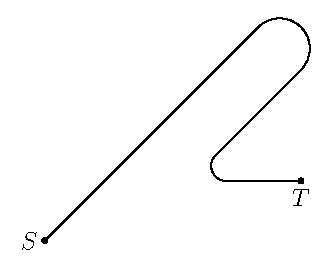
\includegraphics[viewport=234 339 377 452,clip]{nonhol.eps}\\
\caption{ÖʵãÔ˶¯¹ì¼£}\label{figure:coordinate}
\end{figure}

%\vspace*{5mm}
%\centerline{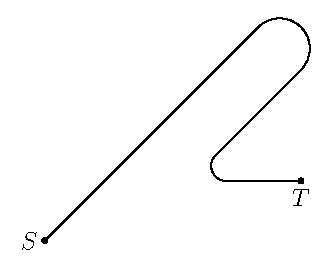
\includegraphics{nonhol.eps}}
%\vskip 2mm
%\centerline{{\footnotesize ͼ1 \quad ÖʵãÔ˶¯¹ì¼£  }}
%\vskip 0.55\baselineskip

Õâ¸öÎÊÌâµÄ¶à½âÐÔ£¬ÊÇÓÉÓÚ²»Í¬ÇéÐÎÏÂÖʵãÊÜÁ¦Çé¿ö²»Í¬¡£Ï£Íûͨ¹ý\eqref{eq:unit}À´ÇóµÃÖʵãËùÊÜÔ¼ÊøÁ¦½ø¶øÇó½âÖʵãµÄÔ˶¯ÊDz»ÄÜʵÏֵģ¬Êµ¼ÊÉÏÎÒÃÇÖ»ÄܽøÐÐÏà·´µÄÇó½â£¬¼´¸ù¾ÝÒÑÖªµÄÔ˶¯¹ì¼£Çó³öÖʵãÊÜÁ¦Çé¿ö¡£
´ÓͼÖÐÒ²¿ÉÒÔ¿´³ö½ö½ö¸ø¶¨³õʼÌõ¼þÒ²ÊDz»¹»µÄ£¬ÏàͬµÄ³õʼÌõ¼þ£¬Ö»ÒªÔ˶¯¹ý³ÌÖÐÊÜÁ¦Çé¿ö²»Í¬£¬¿ÉÒÔ¶ÔÓ¦ÍêÈ«²»Í¬µÄÔ˶¯¡£ÒªÍêÈ«Çó½âÖʵãµÄÔ˶¯£¬±ØÐë¸ø³öÖʵãÔÚÔ˶¯¹ý³ÌÖеÄÊÜÁ¦Çé¿ö¡£Êµ¼ÊÉÏ£¬´ÓÕâ¸öͼҲ¿ÉÒԵõ½£¬Ö»ÒªÓкÏÊʵĿØÖÆ×÷ÓÃÖʵã¿ÉÒÔÔ˶¯µ½¿Õ¼äÖÐÈÎÒâλÖ㬶øÕâÒ²ÕýÊÇ·ÇÍêÕûÔ¼ÊøµÄÌص㡣


ÕâÖÖ¹ÛµãÆäʵ¿ÉÒÔÍƹ㵽ºÜ¶à¾­µä·ÇÍêÕûϵͳÖУ¬ÀýÈçбÃæÉϱùµ¶Ô˶¯ÎÊÌ⣬Á½ÂÖС³µÎÊÌ⣬¸ÕÇòÔÚ´Ö²ÚÃæ´¿¹ö¶¯ÎÊÌâ¡£Âú×ãËüÃǸ÷×Ô·ÇÍêÕû¹ØϵµÄÔ˶¯Óкܶ࣬²»Í¬Ä£Ð͸ø³öµÄ½âʵ¼ÊÉϸ÷×Ô°µº¬ÁËϵͳÊÜÁ¦×´¿ö¡£²»Í¬µÄÊÜÁ¦×´¿öµ±È»¸ø³ö²»Í¬µÄ·½³ÌºÍ²»Í¬µÄ½â£¬¼´Ê¹ËüÃǶ¼»áÂú×ã·ÇÍêÕû¹Øϵ¡£´ÓÕâ¸ö½Ç¶ÈÀ´Ëµ£¬ÎÞÂÛÊÇChetaevÄ£ÐÍ»¹ÊÇVacco¶¯Á¦Ñ§Ä£ÐͶ¼Óë¾­µä·ÖÎöÁ¦Ñ§²»Ã¬¶Ü£¬ËüÃǸø³öµÄ½âÖ»ÒªÊÇÂú×ãËùÒªÇóµÄ·ÇÍêÕû¹Øϵ¾ÍÊÇÕýÈ·µÄ£¬²»Í¬µÄÖ»ÊÇËüÃǸ÷×Ô°µº¬µÄ¿ØÖÆÁ¦¡£ChetaevÌõ¼þ¶ÔÓ¦µÄÕýÊÇÒ»ÖÖ¿ØÖÆÁ¦£¬¼´\eqref{eq:leom}µÄÓҶˣ¬ÔÚÕâÖÖ¿ØÖÆ×÷ÓÃÏ¿ÉÇóµÃϵͳµÄÔ˶¯¡£Ï£Íû¸ù¾ÝÕâ¸öÔ˶¯·´Çó³öËùνµÄ·ÇÍêÕûÔ¼ÊøÁ¦µ±È»Ö»ÄÜÔٴεõ½Õâ¸ö¿ØÖÆÁ¦£¬ÒòΪËüÃDZ¾¾ÍÊÇͬһ¼þÊÂÇé¡£¶øVaccoÄ£ÐÍÔò°µº¬µÄÊÇÁíÒ»ÖÖ¿ØÖÆÁ¦ÇéÐΣ¬ÕâÖÖ¿ØÖÆÁ¦Ê¹µÃϵͳÐÞÕýºóµÄ×÷ÓÃÁ¿È¡×¤Öµ£¬Ô˶¯µÄ¹ì¼£ÊDzâµØ¹ìµÀ¡£ÔÚVaccoÄ£ÐÍÖиüÄÜÌåÏÖ·ÇÍêÕûÁ¦Ñ§ÎÊÌâ±¾ÖÊÊÇ¿ØÖÆÎÊÌâµÄ¹Ûµã¡£ÏÔÈ»ÎÒÃÇÒ²¿ÉÒÔʹÓÃÆäËûÄ£ÐÍ¡£Ö»ÒªÎÒÃǸø¶¨»ò¼ÙÉèÆäËûµÄ¿ØÖÆÁ¦ÇéÐΣ¬ÄÇôµÃµ½µÄ¶¯Á¦Ñ§·½³Ìµ±È»²»Í¬ÓÚÕâÁ½¸öÄ£ÐÍ£¬µ«Ö»Òª²»ÆÆ»µÔ¤ÏÈÒªÇóµÄ·ÇÍêÕû¹ØϵËüÃÇÈÔÈ»ÊÇÕýÈ·µÄ¡£


\section{½áÂÛ}
\label{sec:conclusion}

ÔÚ·ÇÍêÕûϵͳµÄÑо¿ÖУ¬ÍùÍù´æÔÚ´óÁ¿µÄÕùÂÛ£¬ÀýÈçLagrangeÔ­ÀíºÍHamiltonÔ­ÀíµÄÓÐЧÐÔ£¬ÐéλÒƵĶ¨Ò壬΢·Ö±ä·ÖÔËËã½»»»ÐÔµÈÎÊÌâ¡£ÈËÃÇͨ¹ý¶ÔÕâЩÎÊÌâµÄÌÖÂÛ£¬¼ÓÉîÁ˶ԷÇÍêÕûÁ¦Ñ§µÄÈÏʶ£¬Í¬Ê±Ò²µÃµ½Á˺ܶà·ÇÍêÕûϵͳµÄÔ˶¯·½³Ì¡£µ«ÕâЩ·½³ÌÍùÍùÊ®·Ö¸´ÔÓ¶øÄÑÓÚÓ¦Ó㬶øÇÒ¸ù¾Ý²»Í¬µÄÄ£Ð͵õ½µÄ·½³Ì»¹²»Ð­µ÷¡£ÒÑÓеÄì¶ÜºÍÀ§»ó´ÙʹÎÒÃDZØÐè¹Ø×¢·ÇÍêÕûÔ¼ÊøµÄÎïÀíʵÖÊ¡£·ÇÍêÕûÔ¼ÊøÊÇÈçºÎ±»³éÏó³öÀ´£¿·ÇÍêÕûÔ¼Êø¹ØϵÈçºÎʵÏÖ£¿±¾ÎÄÕýÊÇ´ÓÎïÀí±³¾°¶ø²»ÊÇÊýѧ·ÖÎö³ö·¢À´Ì½ÌÖÕâ¸öÎÊÌâ¡£

×÷ΪÀý×Ó£¬±¾ÎÄÏêϸ·ÖÎöÁ˱ùµ¶Ô˶¯½âµÄºÏÀíÐÔ²¢ÌÖÂÛÁ˱ùµ¶Ô˶¯µÄÎïÀíʵÏÖ£¬½âÊÍÁËÔÚ±ùµ¶Ô˶¯ÖгöÏÖµÄËùν·ÇÍêÕûÁ¦»ò¸úËæÁ¦µÄÎïÀíÒâÒå¡£

Õë¶ÔÒ»°ã·ÇÍêÕûϵͳ£¬ÎÒÃÇÌá³öÈçϹ۵㣺

1.ͨ³£Ëù˵µÄ·ÇÍêÕûÔ¼Êø£¬Ó¦µ±³Æ×÷·ÇÍêÕû¹Øϵ£¬ÕâÊÇϵͳÔÚÔ˶¯ÖбØÐëÂú×ãµÄ¹Øϵ£¬¿ÉÒÔ×÷ΪÃèÊöÔ˶¯µÄÌØÕ÷£¬»òÕßÊÇÔ¤Ïȸø¶¨µÄϵͳÔ˶¯µÄÊ״λý·Ö¡£·ÇÍêÕûÔ¼Êø²»¾ß±¸ÍêÕûÔ¼ÊøÔÚ·ÖÎöÁ¦Ñ§ÖеĻù´¡µØλ¡£Æäʵ£¬ÏµÍ³µÄÊ״λý·Ö»òÊغãÁ¿Ò²¿ÉÒÔ¿´×÷ÊÇ·ÇÍêÕûÔ¼Êø,µ«³ýÁËһЩ¼òµ¥µÄÎÊÌ⣬½ö¿¿ÕâЩÊ״λý·Ö²¢²»ÄÜÍêÈ«Çó½âϵͳ¡£Àý\ref{ex:unit}ÕýÊÇÕâÑùµÄÀý×Ó£¬\eqref{eq:unit}¿ÉÒÔÈÏΪÊÇÄÜÁ¿ÊغãÁ¿£¬µ«½öÓÐÕâ¸öÊغãÁ¿²»ÄÜÈ·¶¨ÎÊÌâµÄ½â¡£

2.²»´æÔÚËùνµÄ·ÇÍêÕûÁ¦£¬¼´ÓÉÓÚ·ÇÍêÕûÔ¼Êøµ¼ÖµķÇÍêÕûÔ¼ÊøÁ¦¡£Áîϵͳ±£³Ö·ÇÍêÕû¹ØϵµÄ×÷ÓÃÁ¦ÊÇÍâ½çÊ©¼ÓµÄ¿ØÖÆÁ¦£¬Õâ¸öÁ¦ÐèÒªÃ÷È·¸ø¶¨£¬»òÕßÊǸù¾ÝÒÑÖªÔ˶¯¿ÉÈ·¶¨³öÀ´¡£

3.·ÇÍêÕûϵͳµÄÇó½âÐèÒªÃ÷È·¸ø³öϵͳµÄ³õʼÌõ¼þºÍϵͳµÄÊÜÁ¦×´¿ö£¬Ö»¸ø³ö·ÇÍêÕû¹ØϵµÄϵͳ£¬ÆäÔ˶¯·½³ÌºÍ½âÊDz»È·¶¨µÄ¡£Í¨¹ý²»Í¬Ä£Ð͵õ½µÄ½â¶¼ÊÇ°µº¬ÁËϵͳµÄÊÜÁ¦×´¿ö¡£

4.·ÇÍêÕûϵͳÎÊÌâ±¾ÖÊÉÏÊÇ¿ØÖÆÎÊÌ⣬¼´ÈçºÎÊ©¼Ó¿ØÖÆÁ¦À´Ê¹ÏµÍ³½øÐÐÄ¿±êÔ˶¯¡£

»òÐí´ÓÕâÑùµÄ½Ç¶È¿ÉÒÔ¸üºÃµÄÀí½â·ÇÍêÕûϵͳ£ºÏµÍ³Êܵ½¸÷ÖÖÄÚÁ¦ºÍÍâÁ¦µÄ×÷Óã¬×÷ÓõĽá¹û¡°ÅöÇÉ¡±Ê¹µÃ¹Øϵ\eqref{eq:nhcon}³ÉÁ¢¡£

\refrule

\begin{thebibliography}{999}

\bibitem{1} Hertz H 1894 Die Prizipien der Mechanik in neoen Zusammhage dargestellt (Leipzip: Barth)
\bibitem{2} Mei F X 1985 The Foundations of Mechanics of Nonholonomic System (Beijing: Beijing Institute of Technology Press) (in Chinese) [÷·ïÏè 1985 ·ÇÍêÕûϵͳÁ¦Ñ§»ù´¡ (±±¾©: ±±¾©¹¤ÒµÑ§Ôº³ö°æÉç)]
\bibitem{3} Flannery M 2004 {\it Am. J. Phys.} {\bf 73} 265
\bibitem{4} Flannery M 2011 {\it Am. J. Phys.} {\bf 79} 932
\bibitem{5} Borisov A , Mamaev I 2002 {\it Regular and Chaotic Dynamics} {\bf 7} 43
\bibitem{6} Guo Z H , Gap P Y 1989 {\it Acta Mechanics Sinica} {\bf 5} 253
\bibitem{7} Bloch A 2003 Nonholonomic Mechanics and Control (Interdisciplinary Applied Mathematics Vol 24) (Berlin: Springer)
\bibitem{8} Luo S K , Zhang Y F 2008 Advances in the Study of Dynamics of Constrained Systems (Beijing: Science Press)
\bibitem{9} Greenwood D T 1977 Classical Dynamics (Englewood Cliffs: Prentice-Hall)
\bibitem{10} Neimark J , Fufaev N 1972 Dynamics of Nonholonomic Systems(Transactions of Mathematical Monographs Vol 33)(Providence: American Mathematical Society)
\end{thebibliography}

\newpage

\title{{\boldfont}%
Nonholonomic Mechanics and Control$^{\ast}$}

\author{Wang Dingwen$^{1)\dag}$ \quad  Gao Puyun$^{1)}$}

\email{wangdingwen0618@gmail.com  \quad tel: 15116442661}
\eaddress{1)}{
College of Aerospace Science and Engineering, National University of Defense Technology, Changsha $410072$,China}


\eabstract{The difficult of nonholonomic mechanics is due to the non-integrability of nonholonmic constraints. The origin of nonholonomic constraints is always ignored by researchers. We reveal the control essence of nonholonomic mechanics based on the physical meaning of nonholonomic constraints. From this point of view, the different models( such as Chetaev Model and Vacco Model) can be unified. We clarify that nonholonomic mechanics is still under the theory frame of analytical mechanics. It is the control forces implied by different models that distinguish them.
}
\ekeywords{Nonholonomic Mechanics, Control Theory, Chetaev Model, Vacco Model}


\epacs{45.05.+x,45.20.Jj,45.80.+r}


\newpage
\vspace*{5mm}
\centerline{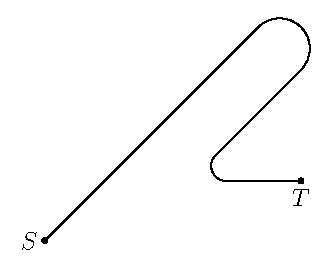
\includegraphics[viewport=234 339 377 452,clip]{nonhol}}
%\vspace*{6mm}
\vskip 2mm
\centerline{{\footnotesize ͼ1 \quad ÖʵãÔ˶¯¹ì¼£}}
\vskip 0.55\baselineskip

\end{document}